%!TEX root = ../../super_main.tex

\section{Vision Representation}
\label{sec:vision_representation}

With the two orientation question, and hereby the four quadrants, decided upon, we have tried to to make two vision representations, namely the metaphor- and the proposition representation.

\subsection{Metaphor Representation}
\label{sub:metaphor_representation}

\begin{figure}[!htbp]
	\centering
	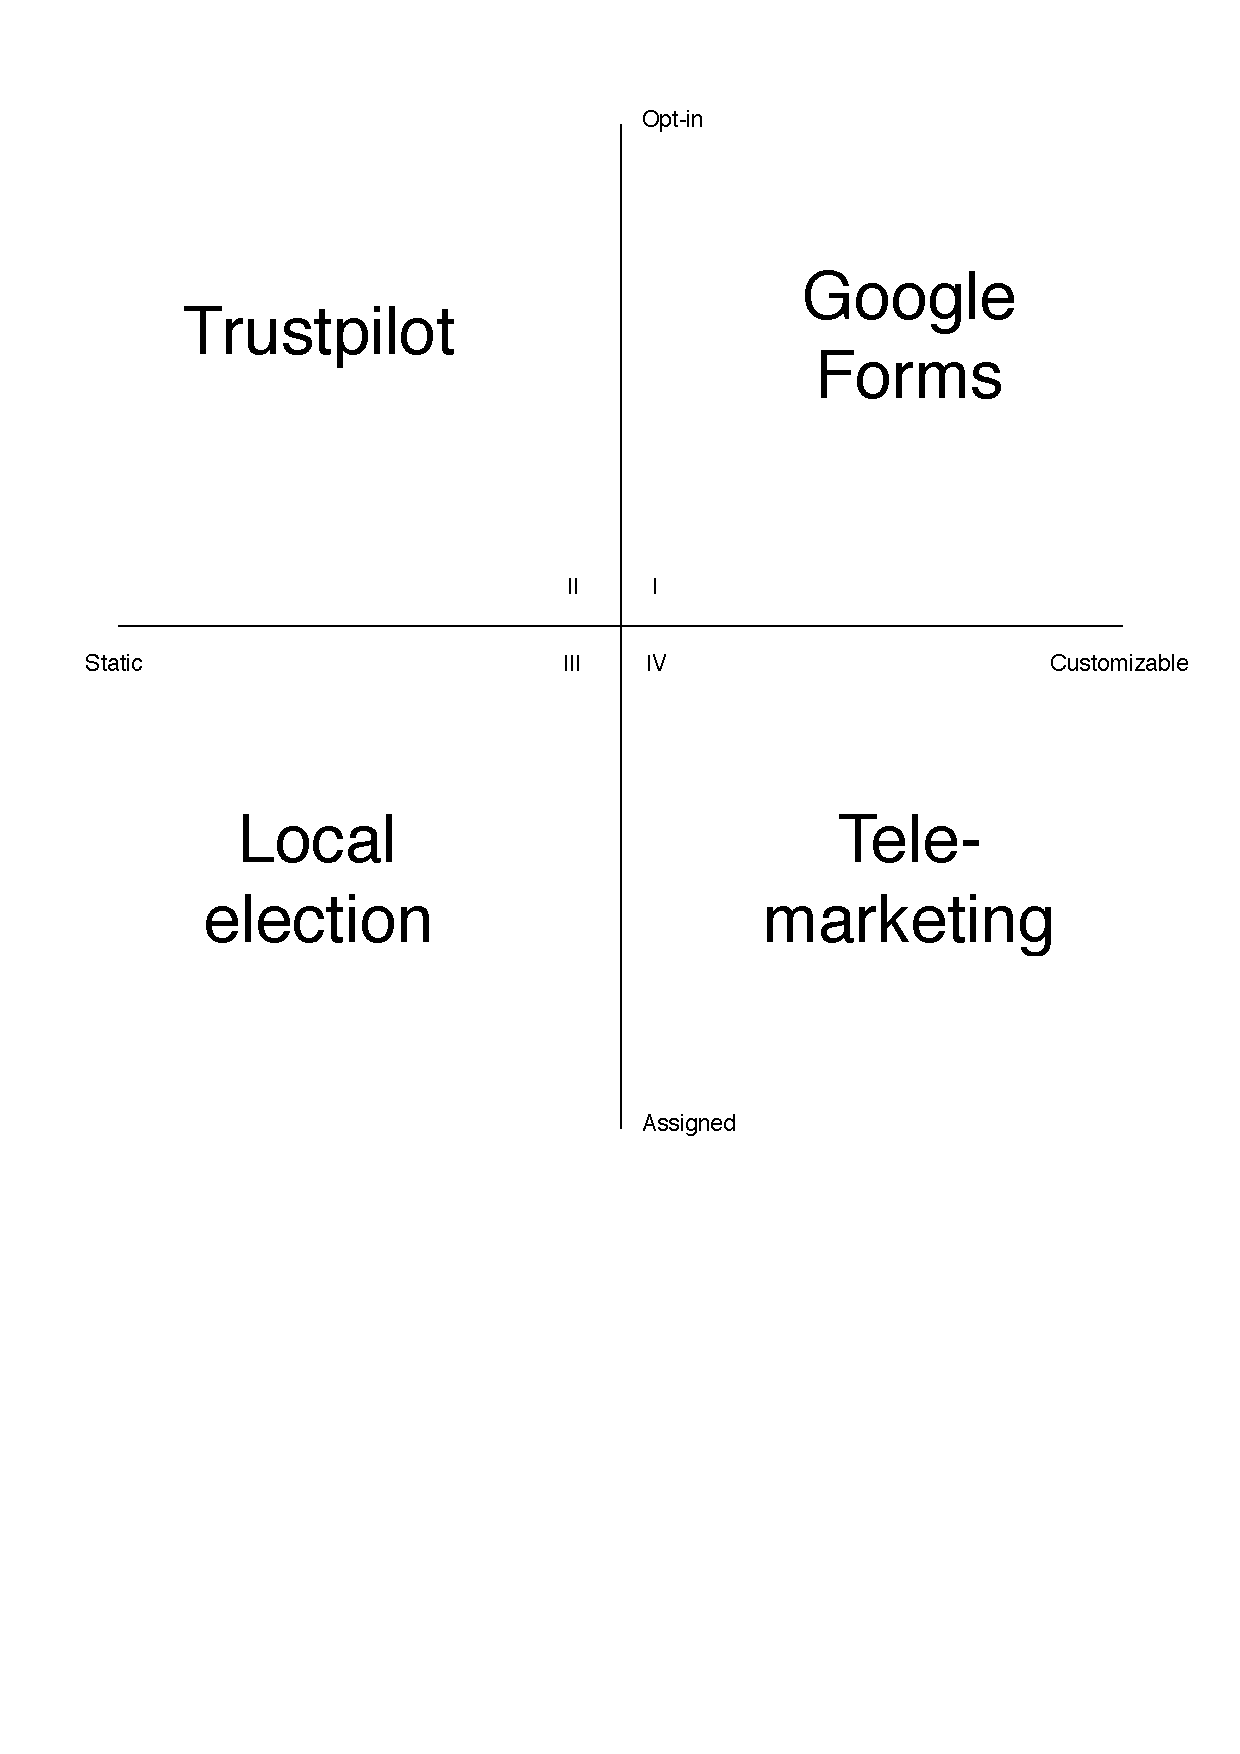
\includegraphics[width=0.8\textwidth]{graphic/problem_analysis/vision/metaphor.pdf}
	\caption{Four metaphors based upon the four quadrants.}
	\label{fig:metaphor}
\end{figure}
\FloatBarrier

\subsection{Proposition Representation}
\label{sub:proposition_representation}

We have tried to define our design idea as propositions, where the propositions can be seen in \figref{fig:proposition}. 
In Essence, a proposition is a statement or assertion that represents a design idea in a literal expression \parencite{essence_book}. Propositions can help to clarify and define scope and focus of the project.

\begin{figure}[!htbp]
	\centering
	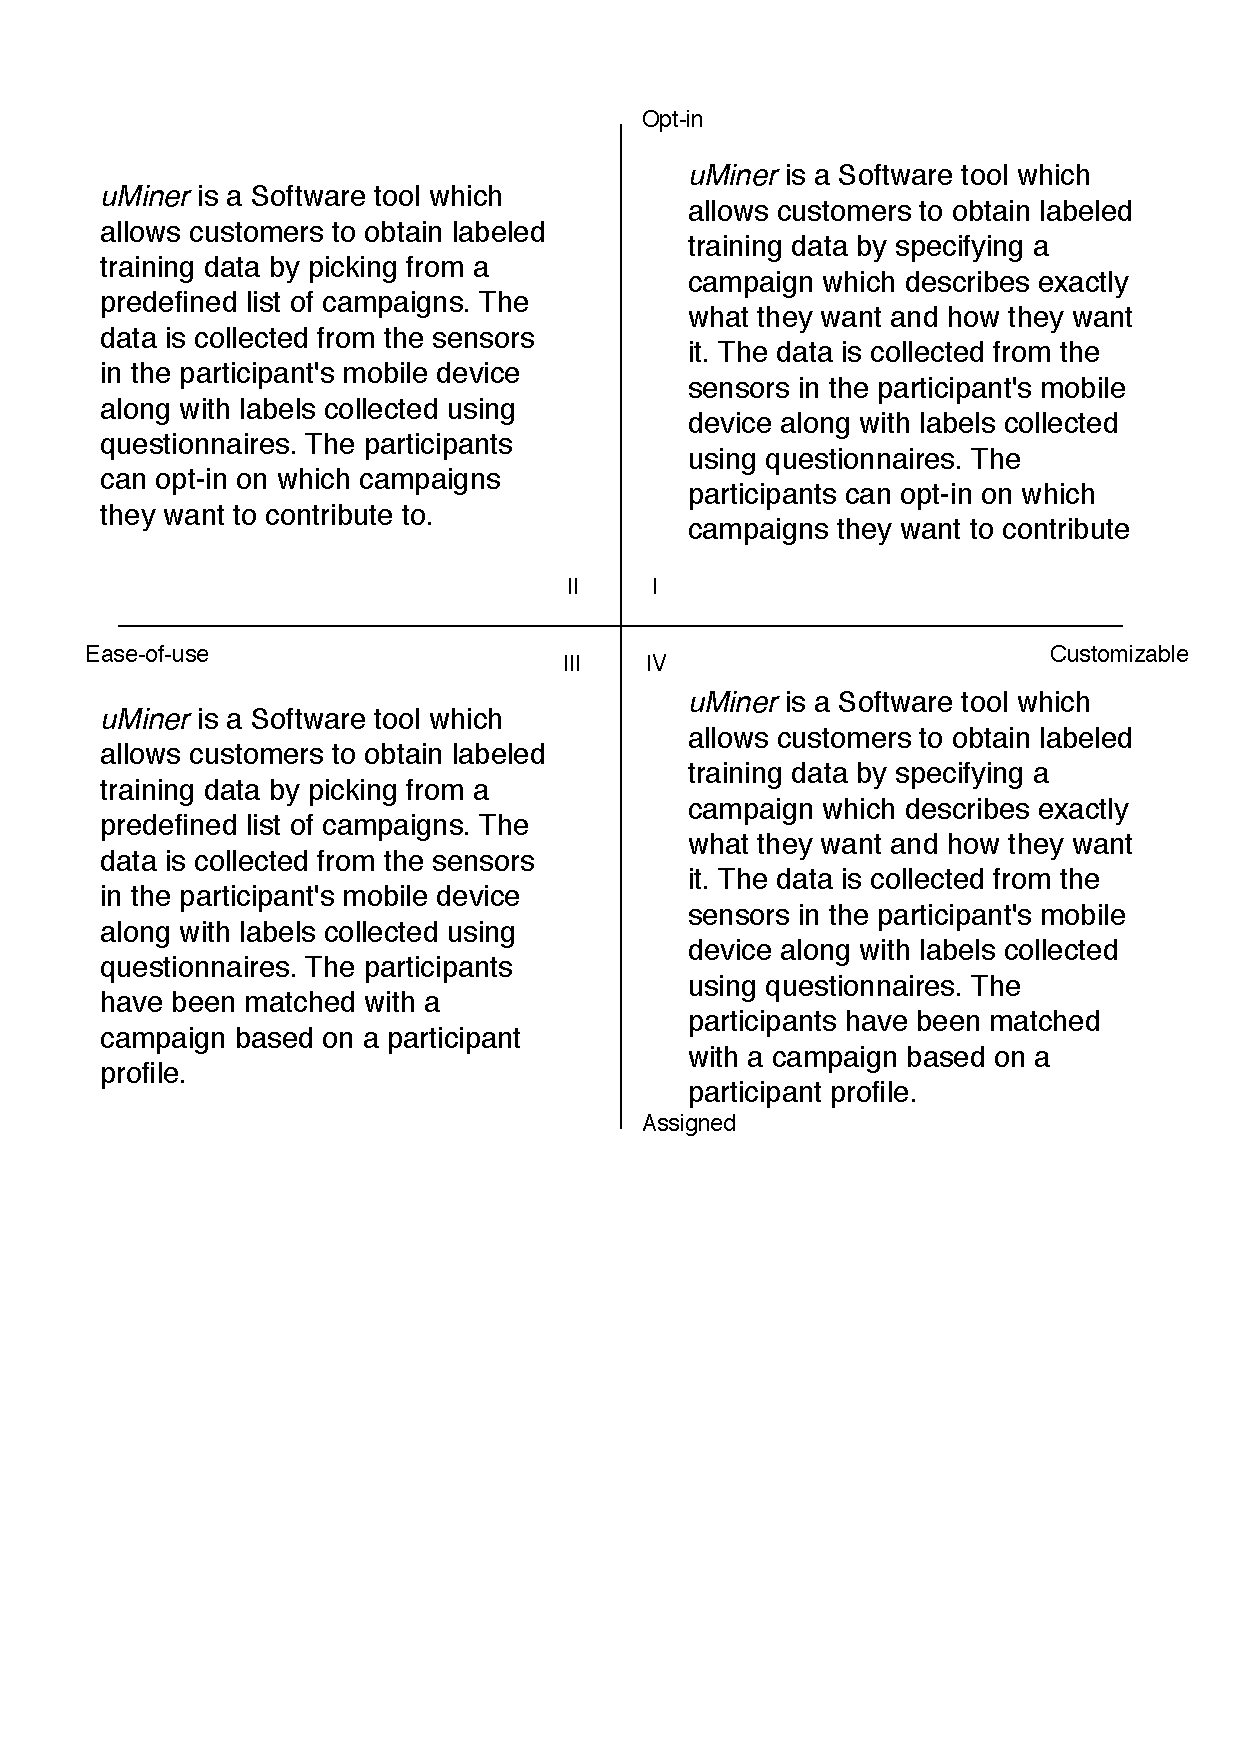
\includegraphics[width=0.8\textwidth]{graphic/problem_analysis/vision/propositions.pdf}
	\caption{Four propositions based upon the four quadrants.}
	\label{fig:proposition}
\end{figure}
\FloatBarrier

The four quadrants agrees on \emph{uMiner} to be a software tool that allows customers to acquire labeled training data. The data is collected using the participant's mobile device, and labels the data using questionnaires. The quadrants vary horizontally between either having a predefined list of campaigns the customers can pick from, or that the customers can specify their own campaigns. The quadrants vary vertically between either by having the participants to be able to opt-in on the campaigns they want to contribute to, or by having a profile for each participant and let their profiles to match with a campaign.

\todo[inline]{Figuren (\figref{fig:system_vision}) skal vist ikke lige stå her, måske i sektionen nedenunder}
\begin{figure}[!htbp]
    \centering
    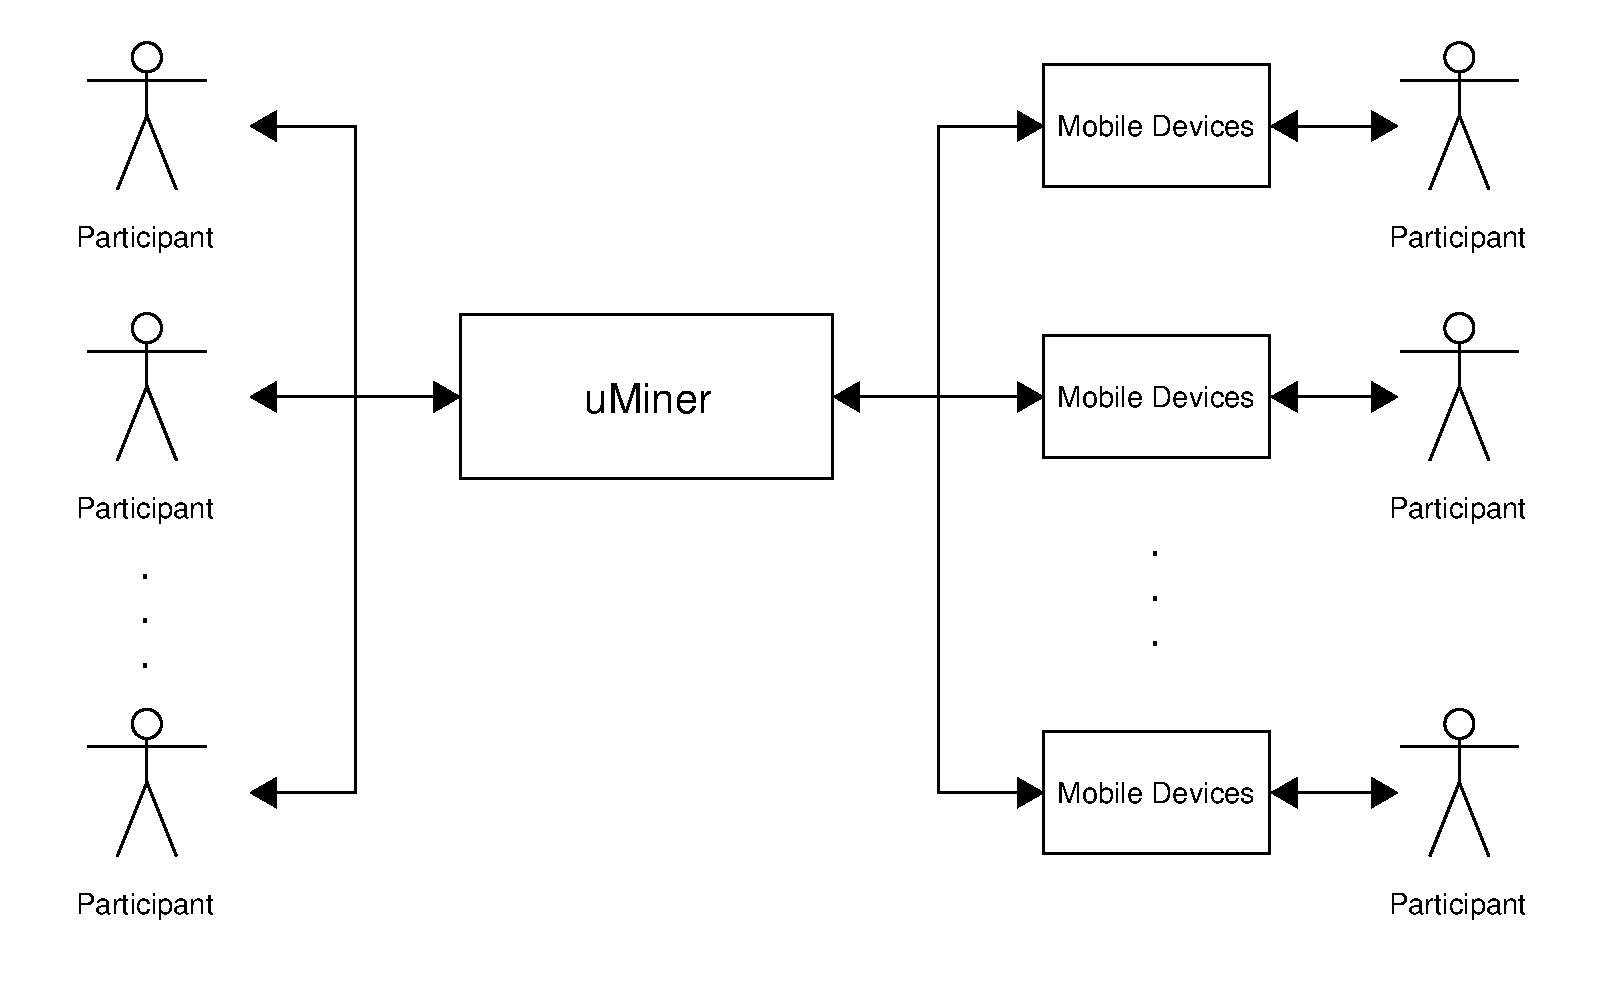
\includegraphics[width=\textwidth]{problem_analysis/vision/system_vision}
    \caption{The system vision.}
    \label{fig:system_vision}
\end{figure}
\FloatBarrier